\section{Electronics}

\F{electronicScheme} shows a schematic diagram of the electronics and readout used for the Cherenkov detector.

The XP4500B Photonis photomultiplier are powered in positive polarity by a CAEN SY4527 outfitted with 1501P boards.

There are two anode signals from the tubes. One of the anode signals is connected directly to Flash ADC
boards built at Jefferson Lab (FADC250)(REF). The FADC sampling frequency is $250 MHz$. The other output is discriminated using a DSC2 unti and connected to CAEN v1190 TDC modules.
The TDCs were set to have 50ps/channel timing resolution.

The Cherenkov FADC250 and TDC information is read out together with the data from the other detector components using the CEBAF Online Data Acquisition system (CODA).

\begin{figure}
	\centering
	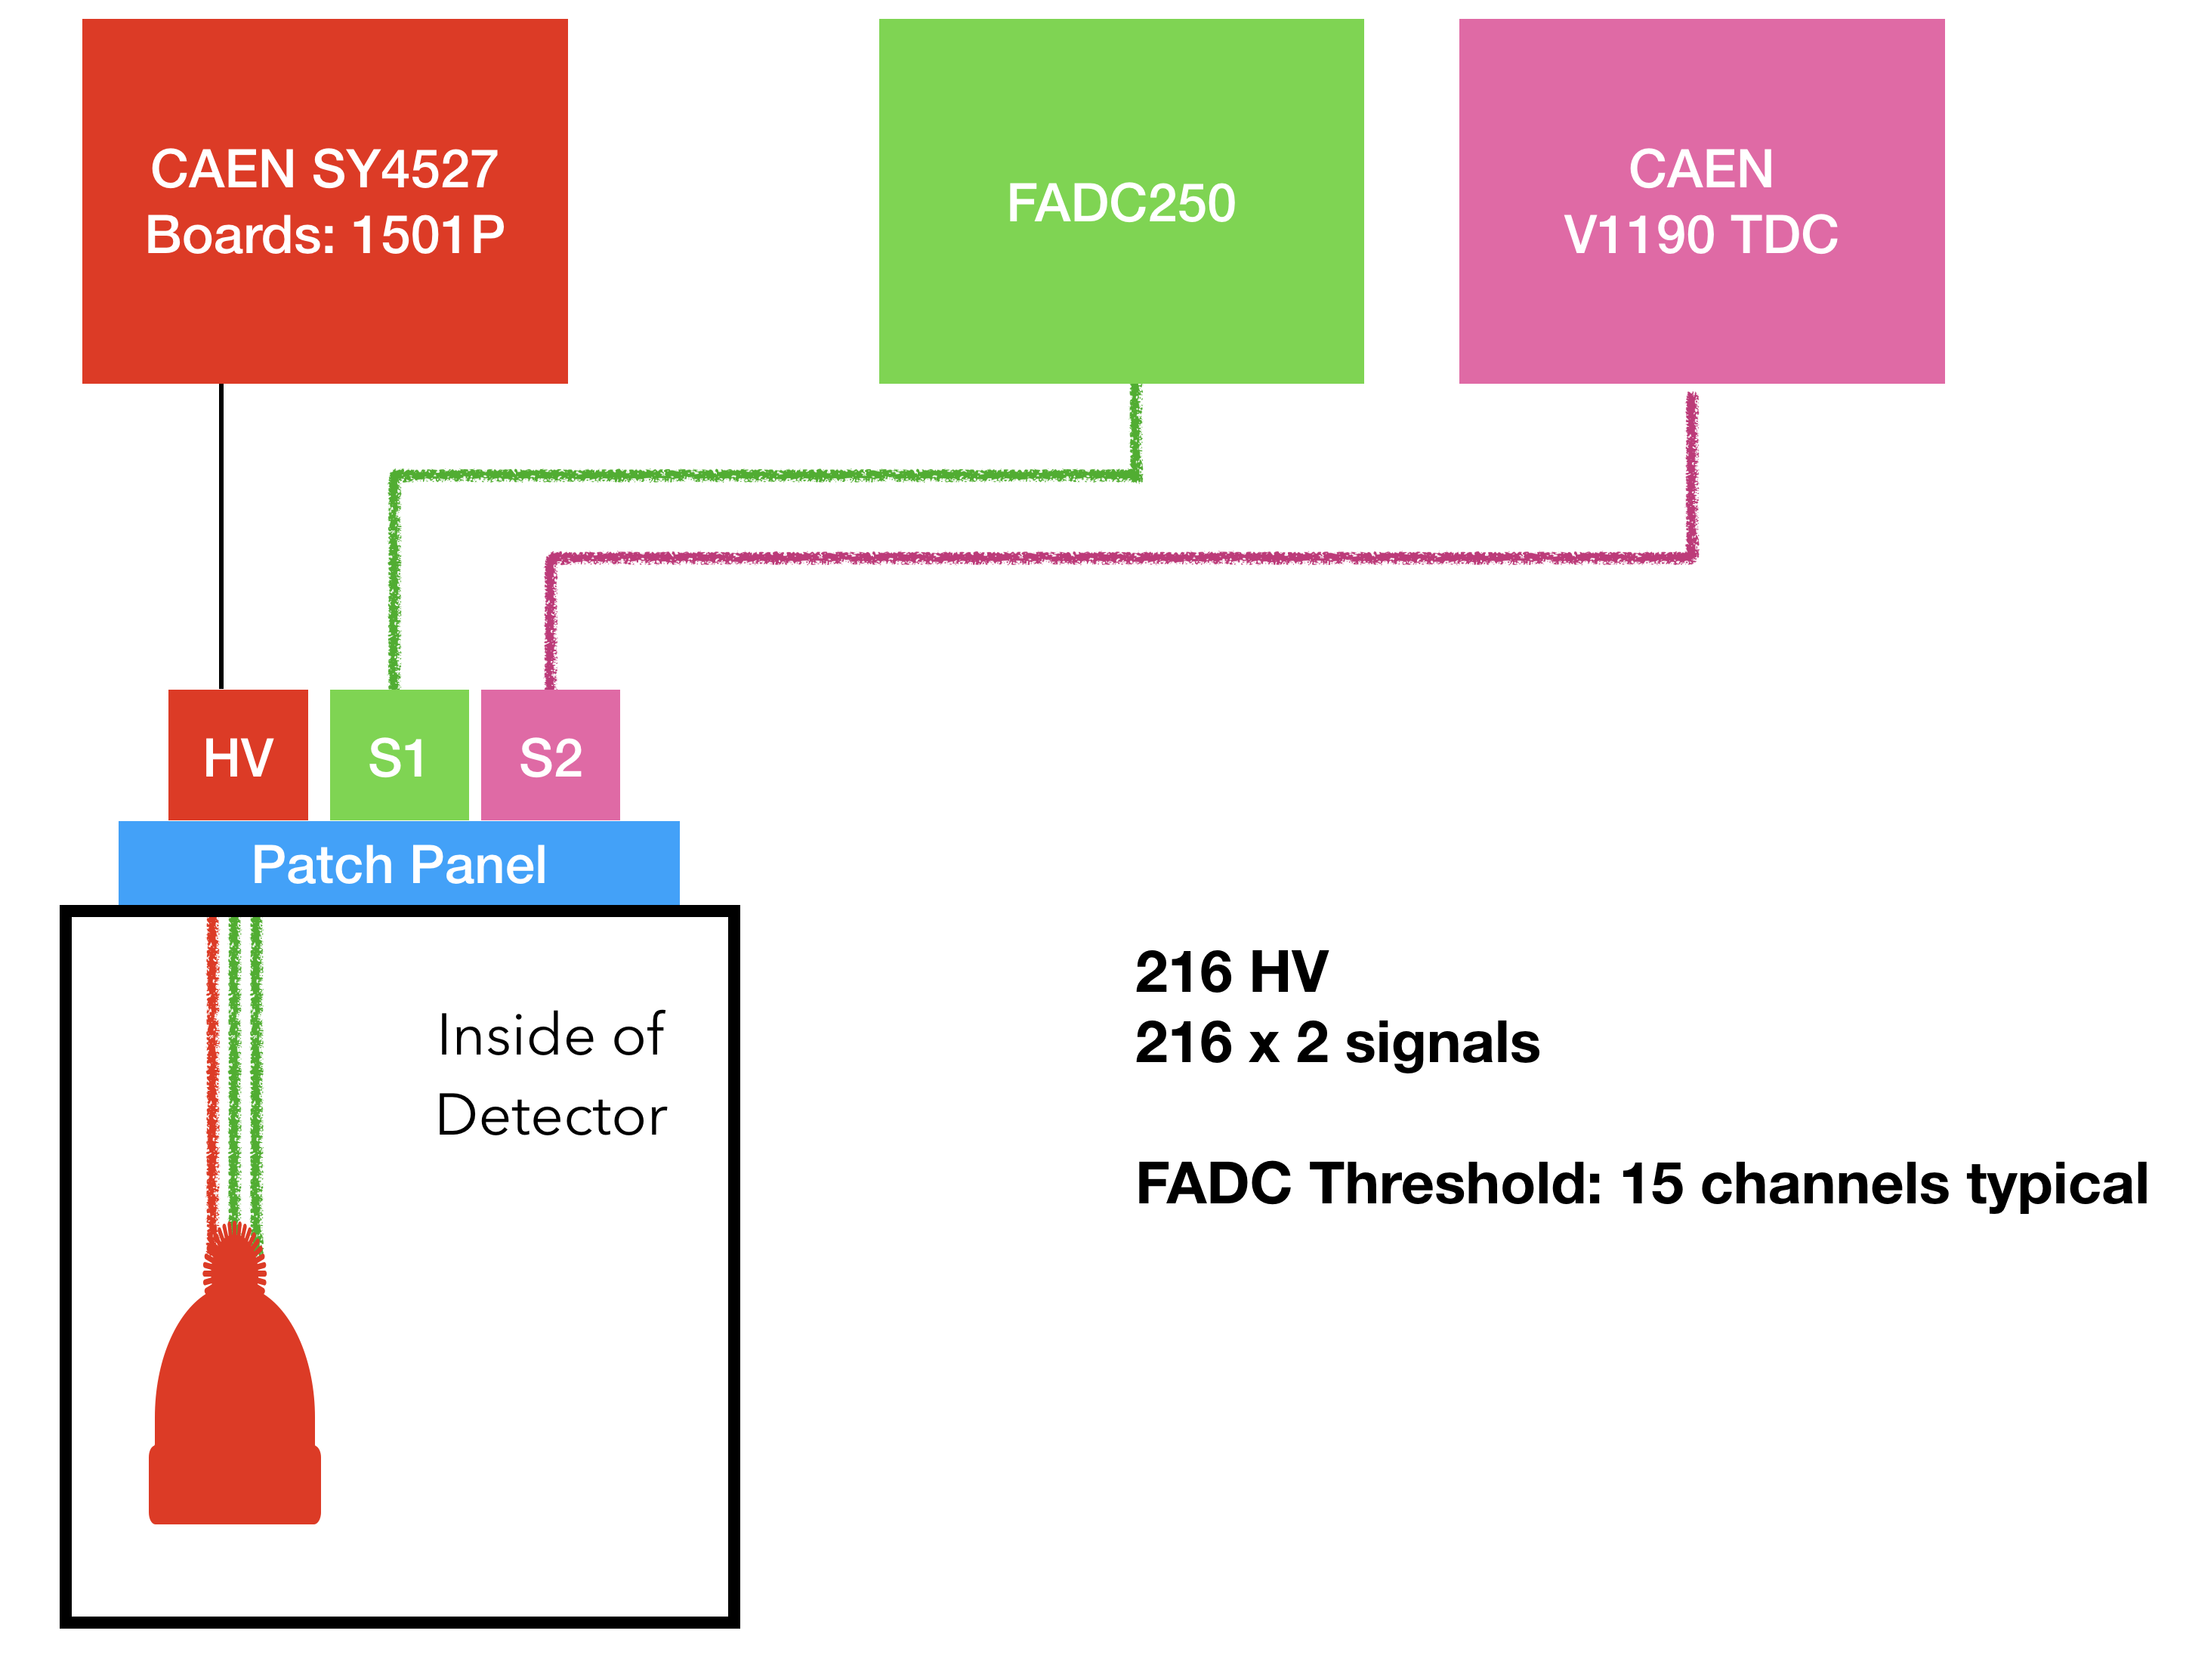
\includegraphics[width=0.95\columnwidth,keepaspectratio]{img/electronicScheme.png}
	\caption{The electronic scheme of the LTCC.}
	\label{fig:electronicScheme}
\end{figure}

\section{Readout}


\subsection{FADC Mode 1 and Mode 7}


In \F{fadc} a typical signal from the FADC250 module is shown. The signal is typically contained in 3-4 time samples (e)ach time samples is 4 ns).
In order to be written to tape, the signal must pass a 30 channels threshold. The FADC250 then consider a time window 12 ns before the sample


\begin{figure}
	\centering
	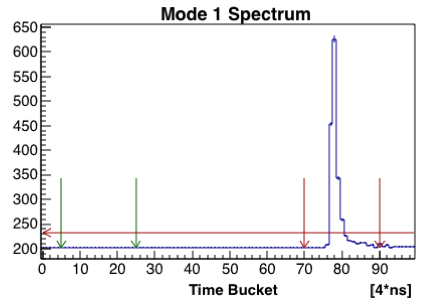
\includegraphics[width=0.95\columnwidth,keepaspectratio]{img/fadc.png}
	\caption{The FADC250 digitized output as a function of sample index from one of the LTCC channel self triggering on the single photo-electron signal.
            The CODA system acquire 100 of these samples if the digitized amplitude passes a 30 channels threshold. The sum of the samples between
				the two arrows results in the integrated charge signal for this event.}
	\label{fig:fadc}
\end{figure}




%\begin{figure}
%	\centering
%	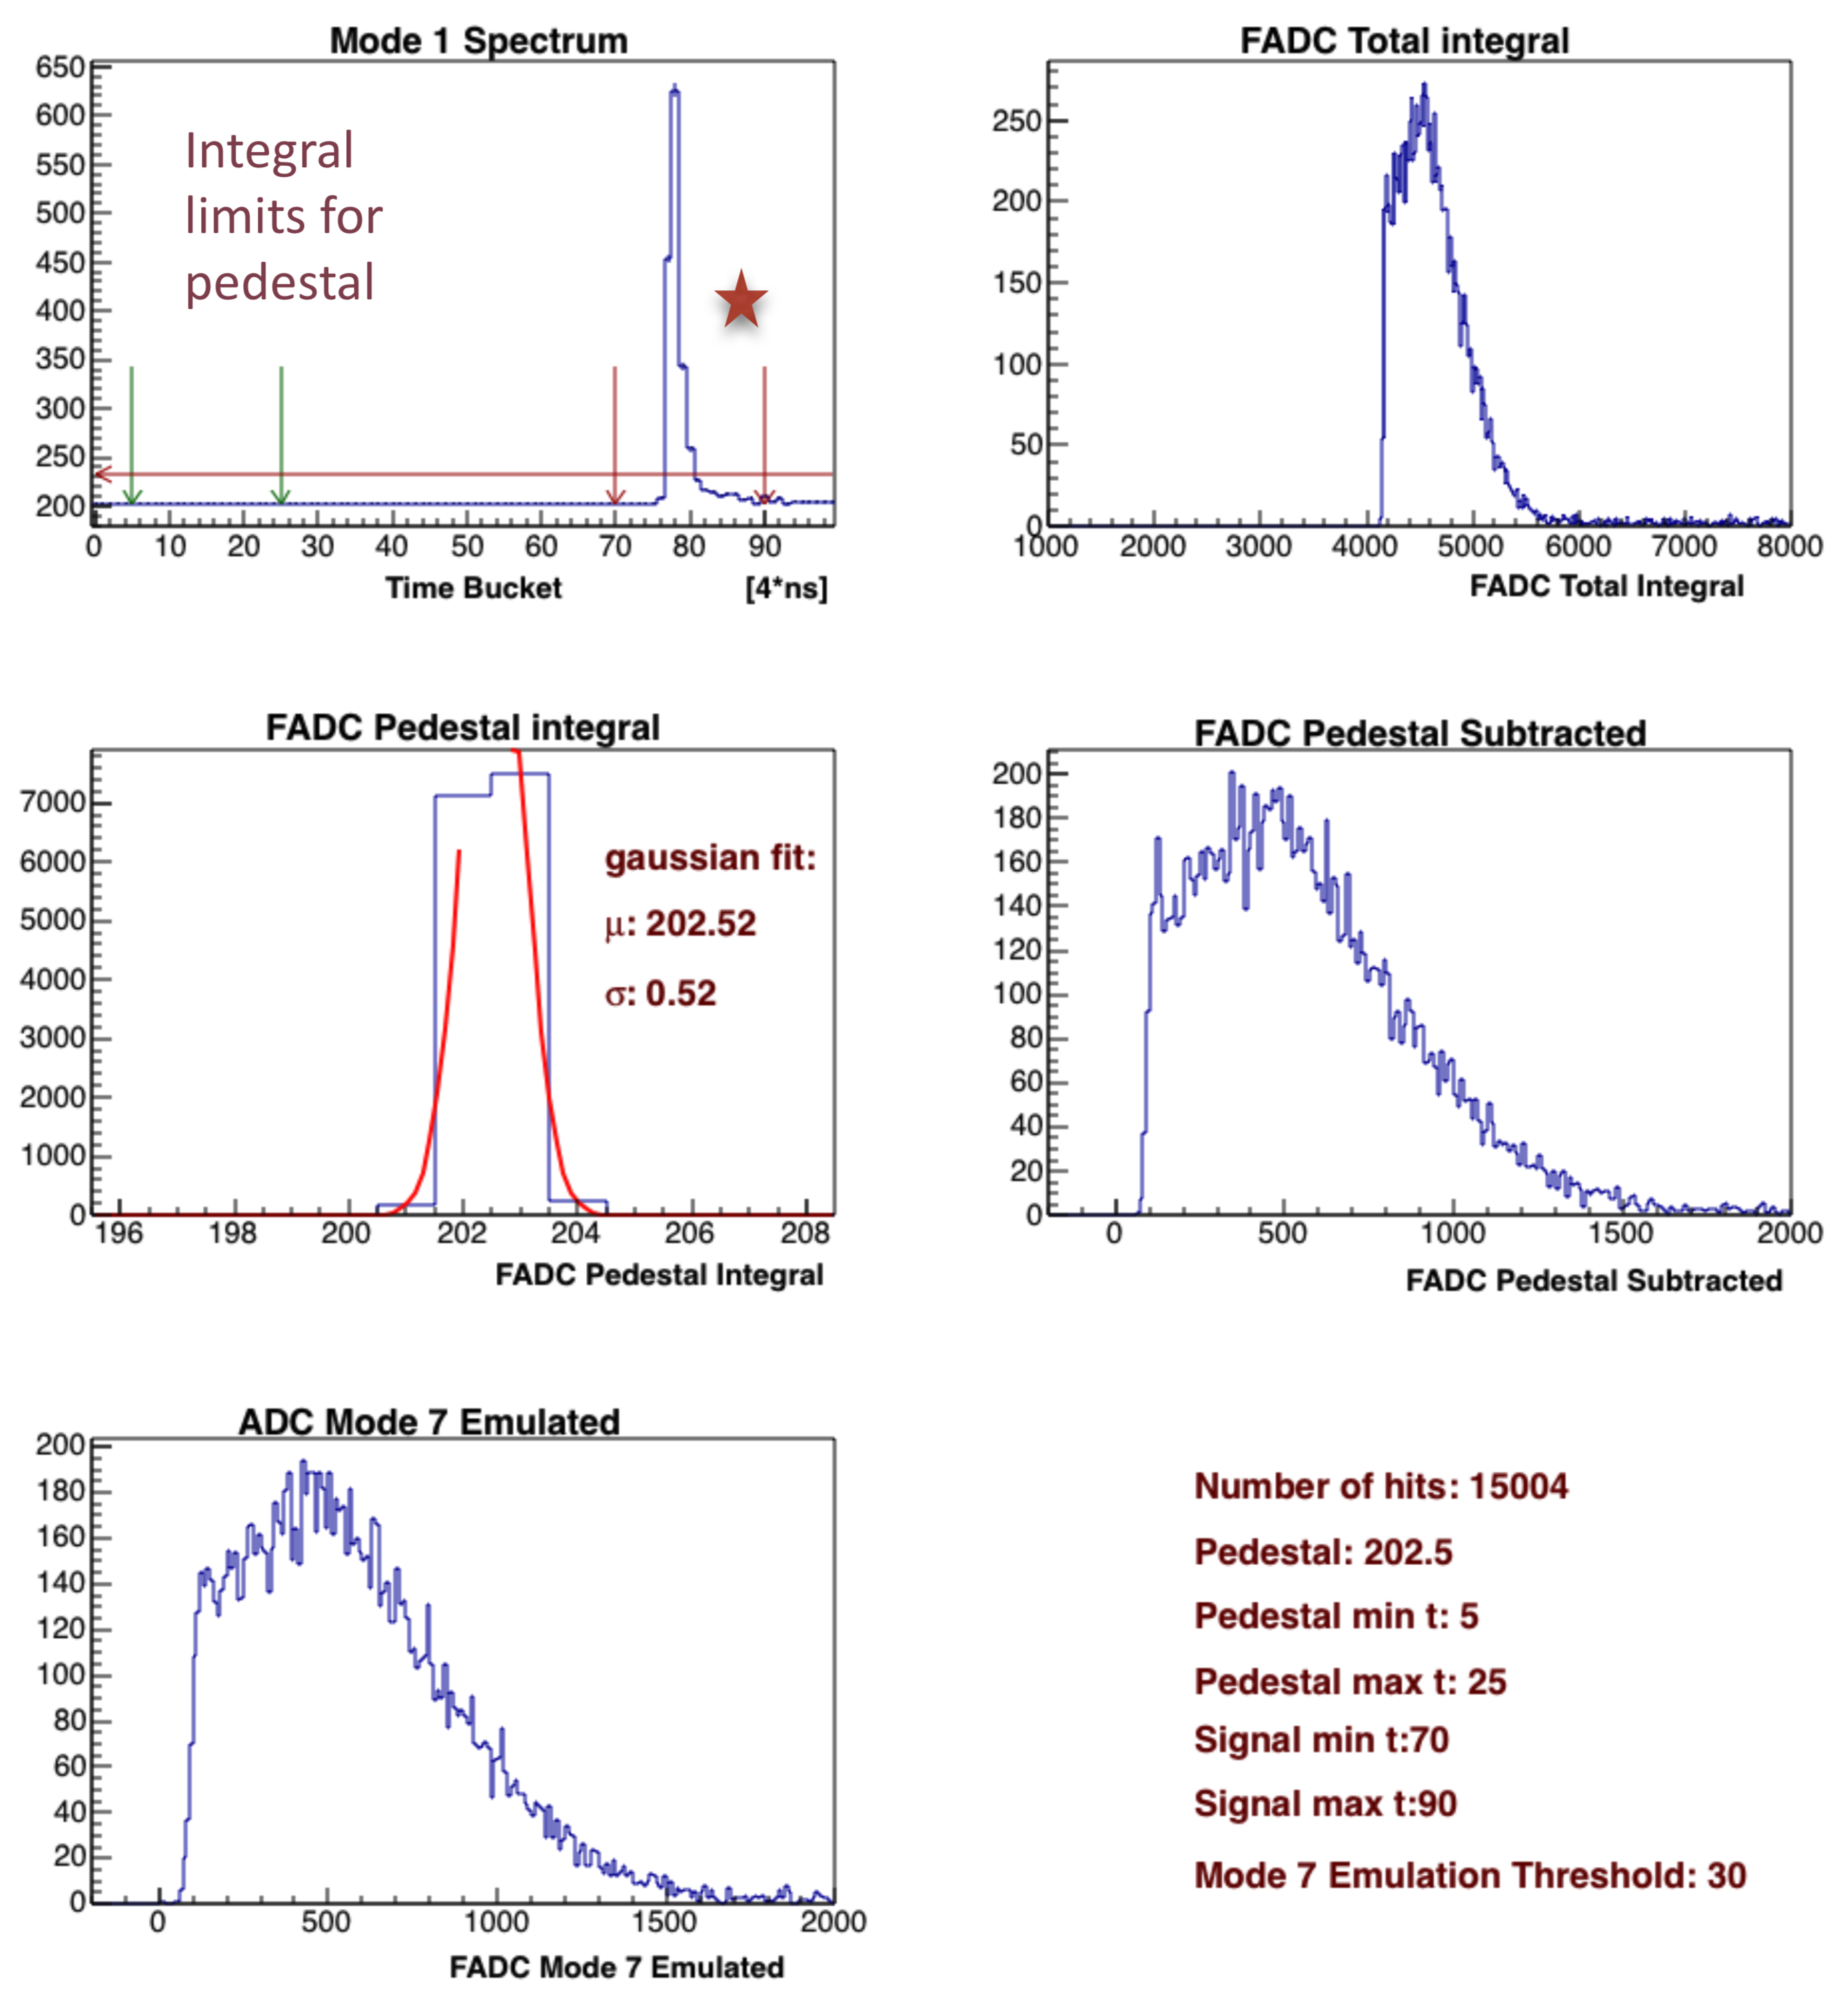
\includegraphics[width=0.95\columnwidth,keepaspectratio]{img/readout.png}
%	\caption{The electronic scheme of the LTCC.}
%	\label{fig:readout}
%\end{figure}
